% Draft of Fig 1.8 (spherical triangle for addition of rotations) in TikZ.
% Same axonometric approach as Fig 1.2.  Build: xelatex Chap1_fig18_draft.tex
%
% Geometry: sphere radius R=4.  Pole N=(0,0,R).
%   V1 = vertex 1: meridian azimuth a2=30, polar angle b2=52  (side N-V1 = beta_2)
%   V2 = vertex 2: meridian azimuth a =62, polar angle b =72  (side N-V2 = beta)
%   side V1-V2 = beta_1 (great-circle arc, angular length ~34.4 deg)
\documentclass[11pt]{article}
\usepackage[a4paper,margin=1.5cm]{geometry}
\usepackage{amsmath}
\usepackage{tikz}
\usetikzlibrary{arrows.meta,math,calc}
\tikzset{
  axo/.style={x={(-0.72cm,-0.46cm)}, y={(1cm,0cm)}, z={(0cm,1cm)}},
  axis/.style={black, thick, -{Latex[length=2.4mm]}},
  side/.style={blue!70!black, line width=1.1pt},          % spherical-triangle sides
  sph/.style={black!55, thin},                            % octant outline
  merid/.style={black!45, thin},                          % meridian/radial construction
  tang/.style={red!80!black, very thick, -{Latex[length=2.2mm]}}, % frame x-axis arrows
  arc/.style={black, thin},
}
\begin{document}
\thispagestyle{empty}
\begin{center}\large\bfseries Fig.~1.8 --- TikZ draft for approval\end{center}
\vspace{1em}
\begin{center}
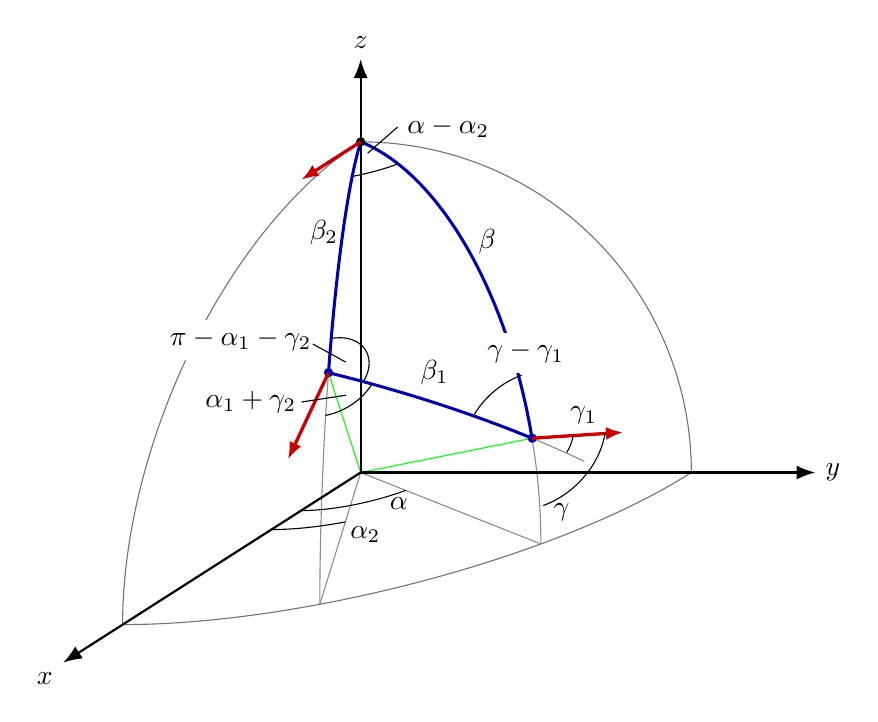
\begin{tikzpicture}[axo, scale=1.05]


  % ---- octant outline of the sphere (R=4) ----
  \draw[sph] plot[variable=\t,domain=0:90,samples=60] ({4*sin(\t)},0,{4*cos(\t)});
  \draw[sph] plot[variable=\t,domain=0:90,samples=60] (0,{4*sin(\t)},{4*cos(\t)});
  \draw[sph] plot[variable=\t,domain=0:90,samples=60] ({4*cos(\t)},{4*sin(\t)},0);
  \pgfmathsetmacro{\rad}{4}
  \pgfmathsetmacro{\at}{30}
  \pgfmathsetmacro{\a}{62.0} 
  \pgfmathsetmacro{\bt}{52.0}
  \pgfmathsetmacro{\b}{72.0} 
  \pgfmathsetmacro{\ct}{-20}
  \pgfmathsetmacro{\c}{72.0} 
  % ---- meridian continuations V1->equator (az 30) and V2->equator (az 62) ----
  \draw[merid] plot[variable=\t,domain=\bt:90,samples=30] ({\rad*sin(\t)*cos(\at)},{\rad*sin(\t)*sin(\at)},{\rad*cos(\t)});
  \draw[merid] plot[variable=\t,domain=\b:90,samples=30] ({\rad*sin(\t)*cos(\a)},{\rad*sin(\t)*sin(\a)},{\rad*cos(\t)});
  % ---- equatorial radial lines O->foot, and the x-axis is the az-0 radial ----
  \draw[merid] (0,0,0)--({\rad*cos(\at)},{\rad*sin(\at)},0);
  \draw[merid] (0,0,0)--({\rad*cos( \a )},{\rad*sin(\a)},0);
  % ---- chords O->V1, O->V2 (position vectors) ----
  \draw[merid,green] (0,0,0)--({\rad*cos(\at)*sin(\bt)},{\rad*sin(\at)*sin(\bt)},{\rad*cos(\bt)});
  \draw[merid,green] (0,0,0)--({\rad*cos(\a)*sin(\b)},{\rad*sin(\a)*sin(\b)},{\rad*cos(\b)});

  % ---- axes ----
  \draw[axis] (0,0,0)--(5,0,0) node[below left]{$x$};
  \draw[axis] (0,0,0)--(0,5.5,0) node[right]{$y$};
  \draw[axis] (0,0,0)--(0,0,5) node[above]{$z$};

  % ---- spherical triangle sides ----
  % N-V1 (beta_2), meridian az 30, polar 0..52
  \draw[side] plot[variable=\t,domain=0:\bt,samples=40] ({\rad*sin(\t)*cos(\at)},{\rad*sin(\t)*sin(\at)},{\rad*cos(\t)});
  % N-V2 (beta), meridian az 62, polar 0..72
  \draw[side] plot[variable=\t,domain=0:\b,samples=40] ({\rad*sin(\t)*cos(\a)},{\rad*sin(\t)*sin(\a)},{\rad*cos(\t)});
  % V1-V2 (beta_1), great-circle slerp, u1=(.682,.394,.616) u2=(.446,.840,.309) Del=34.4 sinDel=.565
  \tikzmath{
    real \uox,\uoy,\uoz; \uox=cos(\at)*sin(\bt); \uoy=sin(\at)*sin(\bt); \uoz=cos(\bt);
    real \utx,\uty,\utz; \utx=cos(\a)*sin(\b);\uty=sin(\a)*sin(\b);\utz=cos(\b);
    real \del; \del=acos(\uox*\utx+\uoy*\uty+\uoz*\utz);
    real \sindel;\sindel=sin(\del);
  }
 % \draw[side] plot[variable=\t,domain=0:1,samples=50] (
 %   {4*(sin((1-\t)*34.4)*0.682+sin(\t*34.4)*0.446)/0.565},
 %   {4*(sin((1-\t)*34.4)*0.394+sin(\t*34.4)*0.840)/0.565},
 %   {4*(sin((1-\t)*34.4)*0.616+sin(\t*34.4)*0.309)/0.565});
 \draw[side] plot[variable=\t,domain=0:1,samples=50] (
    {\rad*(sin((1-\t)*\del)*\uox+sin(\t*\del)*\utx)/\sindel},
    {\rad*(sin((1-\t)*\del)*\uoy+sin(\t*\del)*\uty)/\sindel},
    {\rad*(sin((1-\t)*\del)*\uoz+sin(\t*\del)*\utz)/\sindel});
  \draw[merid] plot[variable=\t,domain=1:1.3,samples=10] (
    {\rad*(sin((1-\t)*\del)*\uox+sin(\t*\del)*\utx)/\sindel},
    {\rad*(sin((1-\t)*\del)*\uoy+sin(\t*\del)*\uty)/\sindel},
    {\rad*(sin((1-\t)*\del)*\uoz+sin(\t*\del)*\utz)/\sindel});
  % ---- vertices ----
  \fill (0,0,4) circle (1.6pt);
  \fill[blue!70!black] (2.729,1.576,2.464) circle (1.6pt);
  \fill[blue!70!black] (1.784,3.359,1.236) circle (1.6pt);

  % ---- frame x'-axis arrows: V1 (south/down), V2 (east/right) ----
  \draw[tang] (0,0,4)--(1,0,4);
  \tikzmath{
    real \uotx, \uoty, \uotz;
    \uotx= cos(\ct)*cos(\at)*cos(\bt)-sin(\ct)*sin(\at);
    \uoty= cos(\ct)*sin(\at)*cos(\bt)+sin(\ct)*cos(\at);
    \uotz= -cos(\ct)*sin(\bt);
  }
  \draw[tang] ($\rad*(\uox,\uoy,\uoz)$)--($\rad*(\uox,\uoy,\uoz)+(\uotx,\uoty,\uotz)$);
   \tikzmath{
    real \uttx, \utty, \uttz;
    \uttx= cos(\c)*cos(\a)*cos(\b)-sin(\c)*sin(\a);
    \utty= cos(\c)*sin(\a)*cos(\b)+sin(\c)*cos(\a);
    \uttz= -cos(\c)*sin(\b);
  } 
  \draw[tang] ($\rad*(\utx,\uty,\utz)$)--($\rad*(\utx,\uty,\utz)+(\uttx,\utty,\uttz)$);

  % ---- angle arcs ----
  % pole angle alpha - alpha2 : latitude arc at polar 12, az at..a
  \draw[arc] plot[variable=\t,domain=\at:\a,samples=20] ({4*sin(12)*cos(\t)},{4*sin(12)*sin(\t)},{4*cos(12)});
  % equatorial azimuths
  \draw[arc] plot[variable=\t,domain=0:\at,samples=20] ({1.5*cos(\t)},{1.5*sin(\t)},0);  % alpha2
  \draw[arc] plot[variable=\t,domain=0:\a,samples=30] ({1.0*cos(\t)},{1.0*sin(\t)},0);  % alpha

  % ---- vertex angle arcs (drawn in the local tangent plane at each vertex) ----
  % tangent directions: toward N (north along meridian), toward the other vertex,
  % south (=-north); the frame x'-arrows are \uot* (at V1) and \utt* (at V2).
  \tikzmath{
    real \nrm,\dprod;
    real \vNax,\vNay,\vNaz,\vPax,\vPay,\vPaz;   % V1: toN, toV2
    \vNax=-\uoz*\uox; \vNay=-\uoz*\uoy; \vNaz=1-\uoz*\uoz;
    \nrm=sqrt(\vNax*\vNax+\vNay*\vNay+\vNaz*\vNaz); \vNax=\vNax/\nrm; \vNay=\vNay/\nrm; \vNaz=\vNaz/\nrm;
    \dprod=\uox*\utx+\uoy*\uty+\uoz*\utz;
    \vPax=\utx-\dprod*\uox; \vPay=\uty-\dprod*\uoy; \vPaz=\utz-\dprod*\uoz;
    \nrm=sqrt(\vPax*\vPax+\vPay*\vPay+\vPaz*\vPaz); \vPax=\vPax/\nrm; \vPay=\vPay/\nrm; \vPaz=\vPaz/\nrm;
    real \vNbx,\vNby,\vNbz,\vPbx,\vPby,\vPbz;   % V2: toN, toV1
    \vNbx=-\utz*\utx; \vNby=-\utz*\uty; \vNbz=1-\utz*\utz;
    \nrm=sqrt(\vNbx*\vNbx+\vNby*\vNby+\vNbz*\vNbz); \vNbx=\vNbx/\nrm; \vNby=\vNby/\nrm; \vNbz=\vNbz/\nrm;
    \vPbx=\uox-\dprod*\utx; \vPby=\uoy-\dprod*\uty; \vPbz=\uoz-\dprod*\utz;
    \nrm=sqrt(\vPbx*\vPbx+\vPby*\vPby+\vPbz*\vPbz); \vPbx=\vPbx/\nrm; \vPby=\vPby/\nrm; \vPbz=\vPbz/\nrm;
    real \pA,\pB,\pC,\pD,\pE,\sA,\sB,\sC,\sD,\sE;
    \pA=acos(\vNax*\vPax+\vNay*\vPay+\vNaz*\vPaz);            % pi-a1-g2 : toN..toV2
    \pB=acos(-\vPax*\vNax-\vPay*\vNay-\vPaz*\vNaz);          % a1+g2 : toV2..south(=-toN)
    \pC=acos(\vNbx*\vPbx+\vNby*\vPby+\vNbz*\vPbz);           % g-g1 : toN..toV1
    \pD=acos(-\vPbx*\uttx-\vPby*\utty-\vPbz*\uttz);          % g1 : (-toV1)..arrow
    \pE=acos(-\uttx*\vNbx-\utty*\vNby-\uttz*\vNbz);          % g : arrow..south(=-toN)
    \sA=sin(\pA); \sB=sin(\pB); \sC=sin(\pC); \sD=sin(\pD); \sE=sin(\pE);
  }
  % V1: pi - alpha1 - gamma2   (toN .. toV2)
  \draw[arc] plot[variable=\s,domain=0:1,samples=24] (
    {\rad*\uox+0.4*(sin((1-\s)*\pA)*\vNax+sin(\s*\pA)*\vPax)/\sA},
    {\rad*\uoy+0.4*(sin((1-\s)*\pA)*\vNay+sin(\s*\pA)*\vPay)/\sA},
    {\rad*\uoz+0.4*(sin((1-\s)*\pA)*\vNaz+sin(\s*\pA)*\vPaz)/\sA});
  % V1: alpha1 + gamma2   (toV2 .. south)
  \draw[arc] plot[variable=\s,domain=0:1,samples=24] (
    {\rad*\uox+0.50*(sin((1-\s)*\pB)*\vPax+sin(\s*\pB)*(-\vNax))/\sB},
    {\rad*\uoy+0.50*(sin((1-\s)*\pB)*\vPay+sin(\s*\pB)*(-\vNay))/\sB},
    {\rad*\uoz+0.50*(sin((1-\s)*\pB)*\vPaz+sin(\s*\pB)*(-\vNaz))/\sB});
  % V2: gamma - gamma1   (toN .. toV1)
  \draw[arc] plot[variable=\s,domain=0:1,samples=24] (
    {\rad*\utx+0.75*(sin((1-\s)*\pC)*\vNbx+sin(\s*\pC)*\vPbx)/\sC},
    {\rad*\uty+0.75*(sin((1-\s)*\pC)*\vNby+sin(\s*\pC)*\vPby)/\sC},
    {\rad*\utz+0.75*(sin((1-\s)*\pC)*\vNbz+sin(\s*\pC)*\vPbz)/\sC});
  % V2: gamma1   ((-toV1) .. arrow)
  \draw[arc] plot[variable=\s,domain=0:1,samples=24] (
    {\rad*\utx+0.45*(sin((1-\s)*\pD)*(-\vPbx)+sin(\s*\pD)*\uttx)/\sD},
    {\rad*\uty+0.45*(sin((1-\s)*\pD)*(-\vPby)+sin(\s*\pD)*\utty)/\sD},
    {\rad*\utz+0.45*(sin((1-\s)*\pD)*(-\vPbz)+sin(\s*\pD)*\uttz)/\sD});
  % V2: gamma   (arrow .. south)
  \draw[arc] plot[variable=\s,domain=0:1,samples=24] (
    {\rad*\utx+0.8*(sin((1-\s)*\pE)*\uttx+sin(\s*\pE)*(-\vNbx))/\sE},
    {\rad*\uty+0.8*(sin((1-\s)*\pE)*\utty+sin(\s*\pE)*(-\vNby))/\sE},
    {\rad*\utz+0.8*(sin((1-\s)*\pE)*\uttz+sin(\s*\pE)*(-\vNbz))/\sE});

  % ---- labels ----
  \node[right] at (0.70,0.95,4.5) {$\alpha-\alpha_2$};
  \draw (0.70,0.95,4.5) to (0.30,0.3,4);
  \node[left]  at (1.40,0.85,3.55) {$\beta_2$};
  \node[right] at (1.10,2.10,3.30) {$\beta$};
  \node[above] at (2.30,2.55,2.) {$\beta_1$};
  % equatorial azimuth labels
  \node at (1.63,1.23,0) {$\alpha_2$};
  \node at (0.82,1.05,0) {$\alpha$};
  % vertex V1 angles
  \node[above left,fill=white]  at (2.75,1.50,2.62) {$\pi-\alpha_1-\gamma_2$};
   \draw (2.75,1.4,2.82) to (2.75,1.8,2.6);
  \node[left]        at (2.45,1.10,1.98) {$\alpha_1+\gamma_2$};
   \draw (2.45,1.05,1.98) to (2.75,1.8,2.2);
  % vertex V2 angles
  \node[above,fill=white]       at (1.95,3.40,2.1) {$\gamma-\gamma_1$};
  \node[right]       at (2.20,4.0,1.7) {$\gamma_1$};
  \node[below right] at (2.20,3.8,0.75) {$\gamma$};
\end{tikzpicture}

\textbf{Fig.~1.8.} Addition of rotations in terms of the spherical geometry.
\end{center}
\end{document}
